  \begin{frame}
  \frametitle{Material para Optical Flow}
  
  \url{https://docs.opencv.org/3.4/d4/dee/tutorial_optical_flow.html}
  \url{https://youtu.be/lnXFcmLB7sM}
  \url{https://www.baeldung.com/cs/motion-field-optical-flow}
  \url{https://rpg.ifi.uzh.ch/docs/teaching/2020/11_tracking.pdf}
  \url{https://rpg.ifi.uzh.ch/teaching.html}
  \url{https://asl.ethz.ch/education/lectures/autonomous_mobile_robots/spring-2021.html}
  \url{https://cs.brown.edu/courses/cs143/2011/results/proj5/gen/}
  \url{https://rpg.ifi.uzh.ch/docs/teaching/2025/03_camera_calibration.pdf}
  \url{https://webdocs.cs.ualberta.ca/~vis/courses/CompVis/lectures13pdf/Lec04OptFlowMot.pdf}
  \url{https://courses.cs.washington.edu/courses/cse576/19sp/notes/Motion19.pdf}

  Flower Garden sequence: \url{https://persci.mit.edu/demos/jwang/garden-layer/orig-seq.html}

  \url{https://cseweb.ucsd.edu/classes/sp19/cse152-a/lec16.pdf}

\end{frame}

\begin{frame}
  \frametitle{Motion Field vs Optical Flow}
  Cuando un objeto se mueve en la escena y es capturado por una cámara, este se proyecta sobre el plano del imagen creando un moviemiento en el plano de la imagen una imagen, al que llamaremos el Motion Field correspondiente a ese punto 3D en movimiento. Desafortunadamente, no es posible garantizar que podamos medir este motion field, todo lo que podemos medir es el movimiento del patrón de brillo en la image, y este se llama Optical Flow.

\end{frame}

% Slide 1
\begin{frame}
  \frametitle{Optical Flow}
  \note{https://youtu.be/lnXFcmLB7sM}

  Method to estimate apparent motion of scene points from a sequence of images.

  Optical flow is the pattern of apparent motion of image objects between two consecutive frames caused by the movement of object or camera. It is 2D vector field where each vector is a displacement vector showing the movement of points from first frame to second.

  Method to estimate the apparent motion of scene points from a sequence of images i.e., the motion of brightness pattern in the image. Each pixel has a vector that tells the optical flow at that point. The motion of the brightness pattern is the optical flow, the length of the vector tells how fast it is moving, and the direction tells its direction on the image plane.

\begin{columns}
  \begin{column}{0.5\textwidth}
    \begin{center}
      \movie[showcontrols,autostart,loop,poster]{\includegraphics[width=0.8\columnwidth]{images/optical_flow/klt_points_video.jpg}}{videos/klt_points.mp4}
      \end{center}
  \end{column}
  \begin{column}{0.5\textwidth}  %%<--- here
    \begin{center}
      \movie[showcontrols,autostart,loop,poster]{\includegraphics[width=\columnwidth]{images/optical_flow/klt_tracking_video.jpg}}{videos/klt_tracking.mp4}
    \end{center}
  \end{column}
\end{columns}

Topics:
\begin{enumerate}
\item Motion Field and Optical Flow
\item Optical Flow Constraint Equation
\item Lucas-Kanade Method
\item Coarse-to-Fine Flow Estimation
\item Applications of Optical Flow
\end{enumerate}
\end{frame}


% Slide 2
\begin{frame}
  \frametitle{Motion Field}
  \begin{center}
    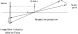
\includegraphics[width=\columnwidth]{./images/optical_flow/motion_field.pdf}
  \end{center}

\end{frame}


\begin{frame}
  \frametitle{Optical Flow}
Motion of brightness patterns in the image.

Ideally: Optical Flow = Motion Field.

\vspace{0.5cm}
\centering
% \includegraphics[width=0.6\textwidth]{placeholder-slide6.png}
\end{frame}

% Slide 4
\begin{frame}
  \frametitle{When is Optical Flow $\neq$ Motion Field?}


  \begin{figure}[!h]
    \subfloat[Motion field]
    {
        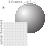
\includegraphics[valign=b,width=0.3\columnwidth]{./images/optical_flow/spinning_sphere_stationary_light.pdf}
    }
    \hspace*{2em}
    \subfloat[Optical Flow]
    {
        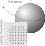
\includegraphics[valign=b,width=0.3\columnwidth]{./images/optical_flow/stationary_sphere_moving_light.pdf}
    }
  \end{figure}

\begin{itemize}
  \item Motion Field exists but no Optical Flow (e.g., spinning sphere, stationary light source)
  \item No Motion Field exists but there is Optical Flow (e.g., stationary sphere, moving light source)
\end{itemize}

\end{frame}

% Slide 3
\begin{frame}
  \frametitle{Optical Flow}
Motion of brightness patterns in the image.

Ideally: Optical Flow = Motion Field.

\vspace{0.5cm}
\centering
% \includegraphics[width=0.6\textwidth]{placeholder-slide6.png}
\end{frame}

% Slide 4
\begin{frame}
  \frametitle{When is Optical Flow $\neq$ Motion Field?}
  \begin{figure}[!h]
    \subfloat[Barber Pole Illusion]
    {
      \movie[showcontrols,autostart,loop,poster]{\includegraphics[valign=m,width=0.2\columnwidth]{./images/optical_flow/barberpole_video.jpg}}{videos/barberpole.mp4}
    }
    \hspace*{2em}
    \subfloat[Motion field]
    {
        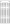
\includegraphics[valign=m,width=0.11\columnwidth]{./images/optical_flow/barberpole_motion_field.pdf}
    }
    \hspace*{2em}
    \subfloat[Optical Flow]
    {
        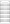
\includegraphics[valign=m,width=0.11\columnwidth]{./images/optical_flow/barberpole_optical_flow.pdf}
    }
  \end{figure}
  \begin{itemize}
    \item Barber Pole Illusion: Motion Field horizontal, Optical Flow appears vertical.
  \end{itemize}
\end{frame}

% Slide 4
\begin{frame}{Point Tracking}
  Problem: given two images, estimate the motion of a pixel point from image $I_0$ to image $I_1$
  
  \begin{center}
    \includegraphics[width=0.3\columnwidth]{./images/optical_flow/point_tracking_1.pdf}
  \end{center}

\end{frame}

% Slide 5
\begin{frame}{Point Tracking}
  Problem: given two images, estimate the motion of a pixel point from image $I_0$ to image $I_1$
  
  \begin{center}
    \includegraphics[width=0.3\columnwidth]{./images/optical_flow/point_tracking_2.pdf}
  \end{center}
\end{frame}

% Slide 6
\begin{frame}{Point Tracking}
  \begin{itemize}
    \item Problem: given two images, estimate the motion of a pixel point from image $I_0$ to image $I_1$
  \end{itemize}

  \begin{center}
    \includegraphics[width=0.3\columnwidth]{./images/optical_flow/point_tracking_3.pdf}
  \end{center}
  
  \begin{itemize}
    \item Two approaches exist, depending on the amount of motion between the frames:
      \begin{itemize}
        \item Block-based methods
        \item Differential methods
      \end{itemize}
  \end{itemize}

\end{frame}

% Slide 7
\begin{frame}{Point Tracking}
  Consider the motion of the following corner
  
  \begin{center}
    \includegraphics[width=0.3\columnwidth]{./images/optical_flow/point_tracking_block_matching_1.pdf}
  \end{center}
\end{frame}

% Slide 8
\begin{frame}{Point Tracking}
  Consider the motion of the following corner
  
  \begin{center}
    \includegraphics[width=0.3\columnwidth]{./images/optical_flow/point_tracking_block_matching_2.pdf}
  \end{center}
\end{frame}

% Slide 9
\begin{frame}{Point Tracking with Block Matching}
  \begin{itemize}
    \item Search for the corresponding patch in a $D \times D$ region around the point to track.
    \item Use SSD, SAD, or NCC.
  \end{itemize}
  
  \begin{center}
    \includegraphics[width=0.3\columnwidth]{./images/optical_flow/point_tracking_block_matching_3.pdf}
  \end{center}
\end{frame}

% Slide 10
\begin{frame}{Pros and Cons of Block Matching}
  \textbf{Pros:}
  \begin{itemize}
    \item Works well if the motion is large
  \end{itemize}
  
  \textbf{Cons:}
  \begin{itemize}
    \item Can become computationally demanding if the motion is large
    \item Can the “search” be implemented in a smart way if the motion is “small”?  
      Yes, use Differential methods
  \end{itemize}
\end{frame}

% Slide 11
\begin{frame}{Point Tracking with Differential Methods}
  Looks at the local brightness changes at the same location. No patch shift is performed!
  
  \begin{center}
    \includegraphics[width=0.3\columnwidth]{./images/optical_flow/point_tracking_differential_methods_1.pdf}
  \end{center}
\end{frame}

% Slide 12
\begin{frame}{Point Tracking with Differential Methods}
  Looks at the local brightness changes at the same location. No patch shift is performed!
  
  \begin{center}
    \includegraphics[width=0.3\columnwidth]{./images/optical_flow/point_tracking_differential_methods_2.pdf}
  \end{center}
\end{frame}

% Slide 13
\begin{frame}{Point Tracking with Differential Methods}
  Looks at the local brightness changes at the same location. No patch shift is performed!
  
  \begin{center}
    \includegraphics[width=0.3\columnwidth]{./images/optical_flow/point_tracking_differential_methods_3.pdf}
  \end{center}
\end{frame}

% Slide 14
\begin{frame}{Point Tracking with Differential Methods}
  Assumptions:

  \begin{columns}
    \begin{column}{0.7\textwidth}
      \begin{itemize}
        \item Brightness constancy: The intensity of the pixels around the point to track does not change much between the two frames
        \item Temporal consistency: The motion displacement is small (1–2 pixels); can be addressed using multi-scale implementations
        \item Spatial coherency: Neighboring pixels undergo similar motion (they all lay on the same 3D surface, i.e., no depth discontinuity)
    \end{itemize}
    \end{column}
    \begin{column}{0.3\textwidth}  %%<--- here
      \begin{center}
      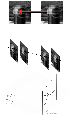
\includegraphics[width=0.7\columnwidth]{./images/optical_flow/point_tracking_differential_methods_properties.pdf}
      \end{center}
    \end{column}
  \end{columns}

\end{frame}


\begin{frame}
  \frametitle{Point Tracking with Differential Methods}
  \begin{figure}[!h]
    \subfloat[]
    {
    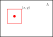
\includegraphics[width=0.4\columnwidth]{./images/optical_flow/klt_displacement_1.pdf}
    }
    \hspace*{2em}
    \subfloat[]
    {
    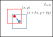
\includegraphics[width=0.4\columnwidth]{./images/optical_flow/klt_displacement_2.pdf}
    }
  \end{figure}

  \begin{center}
    Displacement: $(\delta x, \delta y)$ \hspace*{2em} Optical Flow: $(u,v) = \left(\dfrac{\delta x}{\delta t}, \dfrac{\delta y}{\delta t}\right)$
  \end{center}

\end{frame}


\begin{frame}
  \frametitle{Point Tracking with Differential Methods}

  \begin{figure}[!h]
    \subfloat[]
    {
    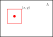
\includegraphics[width=0.4\columnwidth]{./images/optical_flow/klt_displacement_1.pdf}
    }
    \hspace*{2em}
    \subfloat[]
    {
    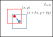
\includegraphics[width=0.4\columnwidth]{./images/optical_flow/klt_displacement_2.pdf}
    }
  \end{figure}

  Assumpion \#1:
  Brightness of image point remains constant over time

  \begin{equation*}
    I(x + \delta x, y + \delta y, t + \delta t) = I(x, y, t)
  \end{equation*}

\end{frame}

\begin{frame}
  \frametitle{Taylor Series Expansion}

  Expand a function as an infinite sum of its derivatives

  \[
  f(x + \delta x) = f(x) + \frac{\partial f}{\partial x}\delta x + 
  \frac{\partial^2 f}{\partial x^2}\frac{\delta x^2}{2!} + \cdots + 
  \frac{\partial^n f}{\partial x^n}\frac{\delta x^n}{n!}
  \]

  If $\delta x$ is small:

  \[
  f(x + \delta x) = f(x) + \frac{\partial f}{\partial x}\delta x + 
  \boxed{O(\delta x^2)} \rightarrow \text{Almost Zero}
  \]

  For a function of three variables with small $\delta x, \delta y, \delta t$:

  \[
  f(x + \delta x, y + \delta y, t + \delta t) \approx f(x, y, t) + 
  \frac{\partial f}{\partial x}\delta x + 
  \frac{\partial f}{\partial y}\delta y + 
  \frac{\partial f}{\partial t}\delta t
  \]
\end{frame}


\begin{frame}
  \frametitle{Point Tracking with Differential Methods}

  \begin{figure}[!h]
    \subfloat[]
    {
    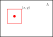
\includegraphics[width=0.4\columnwidth]{./images/optical_flow/klt_displacement_1.pdf}
    }
    \hspace*{2em}
    \subfloat[]
    {
    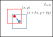
\includegraphics[width=0.4\columnwidth]{./images/optical_flow/klt_displacement_2.pdf}
    }
  \end{figure}

  Assumpion \#2:
  Displacement $(\delta x, \delta y)$ and time step $\delta t$ are small
  (Aplicamos taylor)
  \begin{equation*}
    I(x + \delta x, y + \delta y, t + \delta t) = I(x, y, t) + \dfrac{\partial I}{\partial x} \delta x + \dfrac{\partial I}{\partial y} \delta y + \dfrac{\partial I}{\partial t} \delta t
  \end{equation*}


  \begin{equation*}
    \boxed{I(x+\delta x, y+\delta y, t+\delta t) \approx I(x,y,t) + I_x \delta x + I_y \delta y + I_t \delta t}
  \end{equation*}
\end{frame}

\begin{frame}
  \frametitle{Optical Flow Constraint Equation}

  \begin{equation}\label{eq:uno}
    I(x + \delta x, y + \delta y, t + \delta t) = I(x, y, t)
  \end{equation}
  \begin{equation}\label{eq:dos}
    I(x + \delta x, y + \delta y, t + \delta t) = I(x, y, t) + I_x \delta x + I_y \delta y + I_t \delta t
  \end{equation}
  Subtract \eqref{eq:uno} from \eqref{eq:dos}: \quad 
  \[
  I_x \delta x + I_y \delta y + I_t \delta t = 0
  \]
  Divide by $\delta t$ and take limit as $\delta t \rightarrow 0$: \quad 
  \[
  I_x \frac{\partial x}{\partial t} + I_y \frac{\partial y}{\partial t} + I_t = 0
  \]

  Constraint Equation: \quad \boxed{I_x u + I_y v + I_t = 0} \quad $(u,v)$: Optical Flow

  \[
  (I_x, I_y, I_t) \text{ can be easily computed from two frames}
  \]

\end{frame}

%------------------------------------------------
\begin{frame}
  \frametitle{Computing Partial Derivatives $I_x, I_y, I_t$}

  \begin{center}
    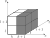
\includegraphics[width=0.35\columnwidth]{./images/optical_flow/computing_partial_derivatives.pdf}
  \end{center}
  %
  \[
  I_x(k, l, t) = \frac{1}{4} [I(k+1,l,t) + I(k+1,l,t+1) + I(k+1,l+1,t) + I(k+1,l+1,t+1)]
  \]
  \[
  - \frac{1}{4}[I(k,l,t) + I(k,l,t+1) + I(k,l+1,t) + I(k,l+1,t+1)]
  \]

  Similarly find $I_y(k,l,t)$ and $I_t(k,l,t)$

\end{frame}

\begin{frame}
  \frametitle{Geometric Interpretation}

  \begin{columns}
    \begin{column}{0.6\textwidth}  %%<--- here
      For any point $(x,y)$ in the image, its optical flow $(u,v)$ lies on the line:
      \[
      I_x u + I_y v + I_t = 0
      \]

      Optical Flow can be split into two components.

      \[
      \mathbf{u} = \mathbf{u}_n + \mathbf{u}_p
      \]

      $\mathbf{u}_n$: Normal Flow \\
      $\mathbf{u}_p$: Parallel Flow
    \end{column}
    \begin{column}{0.4\textwidth}
      \begin{center}
        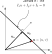
\includegraphics[width=\columnwidth]{./images/optical_flow/optical_flow_geometric_interpretation.pdf}
      \end{center}
    \end{column}
  \end{columns}
\end{frame}

\begin{frame}
  \frametitle{Normal Flow}

  \begin{columns}
    \begin{column}{0.6\textwidth}  %%<--- here
      Direction of Normal Flow:

      Unit vector perpendicular to the constraint line:
      \[
      \hat{\mathbf{u}}_n = \frac{(I_x, I_y)}{\sqrt{I_x^2 + I_y^2}}
      \]

      Magnitude of Normal Flow:

      Distance of origin from the constraint line:
      \[
      |\mathbf{u}_n| = \frac{|I_t|}{\sqrt{I_x^2 + I_y^2}}
      \]

      \[
      \boxed{\mathbf{u}_n = \frac{|I_t|}{(I_x^2 + I_y^2)} (I_x, I_y)}
      \]
    \end{column}
    \begin{column}{0.4\textwidth}
      \begin{center}
        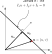
\includegraphics[width=\columnwidth]{./images/optical_flow/optical_flow_geometric_interpretation.pdf}
      \end{center}
    \end{column}
  \end{columns}

\end{frame}

\begin{frame}
  \frametitle{Aperture Problem}
  \begin{center}
    \only<1>{\includegraphics[width=0.35\columnwidth]{./images/optical_flow/aperture_problem_frame_1.pdf}}

    \only<2>{\includegraphics[width=0.35\columnwidth]{./images/optical_flow/aperture_problem_frame_2.pdf}}

    \only<3>{
\includegraphics[width=0.35\columnwidth]{./images/optical_flow/aperture_problem_normal_flow.pdf}}

    \only<4>{\includegraphics[width=0.35\columnwidth]{./images/optical_flow/aperture_problem_actual_motion.pdf}}

  \end{center}
\end{frame}

\begin{frame}
  \frametitle{Aperture Problem}
  \begin{figure}[!h]
    \subfloat[]
    {
      \movie[showcontrols,autostart,loop,poster]{\includegraphics[valign=b,width=0.2\columnwidth]{./images/optical_flow/barberpole_illusion_video.jpg}}{videos/barberpole_illusion.mp4}
    }
    \hspace*{2em}
    \subfloat[]
    {
      \movie[showcontrols,autostart,loop,poster]{\includegraphics[valign=b,width=0.2\columnwidth]{./images/optical_flow/barberpole_aperture_problem_video.jpg}}{videos/barberpole_aperture_problem.mp4}
    }
  \end{figure}
  \begin{itemize}
    \item The aperture problem. The grating appears to be moving down and to the right, perpendicular to the orientation of the bars. But it could be moving in many other directions, such as only down, or only to the right. It is impossible to determine unless the ends of the bars become visible in the aperture.
  \end{itemize}
\end{frame}

% Slide 5
\begin{frame}
  \frametitle{Motion Illusions}
  \begin{itemize}
    \item Donguri Wave Illusion: Static image but perceived motion.
    \item Ouchi Pattern: Inner disc appears to move with respect to the ring.
  \end{itemize}

  \vspace{0.5cm}
  \centering
  % \includegraphics[width=0.6\textwidth]{placeholder-slide9.png}
\end{frame}

% Slide 9
\begin{frame}
  \frametitle{Normal Flow and Aperture Problem}
  \begin{itemize}
    \item Constraint equation gives only a line in $(u,v)$ space.
    \item Can compute normal flow but not full optical flow.
    \item Locally, humans also perceive only normal flow (aperture problem).
  \end{itemize}

  \vspace{0.5cm}
  \centering
  % \includegraphics[width=0.6\textwidth]{placeholder-slide22.png}
\end{frame}

%------------------------------------------------
\begin{frame}
  \frametitle{Optical Flow is Under Constrained}

  Constraint Equation: \quad \boxed{I_x u + I_y v + I_t = 0}

  \vspace{0.5cm}
  2 unknowns, 1 equation.

  \vspace{1cm}
  We need additional constraints.

\end{frame}

%------------------------------------------------
\begin{frame}
  \frametitle{Lucas-Kanade Solution}

  Assumption: For each pixel, assume Motion Field, and hence Optical Flow $(u,v)$, is constant within a small neighborhood $W$.

  % \begin{center}
  % \includegraphics[width=0.55\textwidth]{placeholder}
  % \end{center}

  That is for all points $(k,l) \in W$:
  \[
  I_x(k,l)u + I_y(k,l)v + I_t(k,l) = 0
  \]

\end{frame}

%------------------------------------------------
\begin{frame}
  \frametitle{Lucas-Kanade Solution}

  For all points $(k,l) \in W$: \quad 
  $I_x(k,l)u + I_y(k,l)v + I_t(k,l) = 0$

  Let the size of window $W$ be $n \times n$

  In matrix form:

  \[
  \left[
  \begin{array}{cc}
  I_x(1,1) & I_y(1,1) \\
  I_x(k,l) & I_y(k,l) \\
  \vdots & \vdots \\
  I_x(n,n) & I_y(n,n)
  \end{array}
  \right]
  \left[
  \begin{array}{c}
  u \\
  v
  \end{array}
  \right]
  =
  \left[
  \begin{array}{c}
  -I_t(1,1) \\
  -I_t(k,l) \\
  \vdots \\
  -I_t(n,n)
  \end{array}
  \right]
  \]

  $A$ (Known) $n^2\times2$
  \hspace{0.5cm}
  $\mathbf{u}$ (Unknown) $2\times1$
  \hspace{0.5cm}
  $B$ (Known) $n^2\times1$

  \vspace{0.2cm}
  $n^2$ Equations, 2 Unknowns: Find Least Squares Solution

\end{frame}

%------------------------------------------------
\begin{frame}
  \frametitle{Least Squares Solution}

  Solve linear system: \quad $\mathbf{A u = B}$

  \[
  \mathbf{A^T A u = A^T B} \hspace{1cm} \text{(Least-Squares using Pseudo-Inverse)}
  \]

  In matrix form:

  \[
  \boxed{
  \begin{bmatrix}
  \sum_W I_x I_x & \sum_W I_x I_y \\
  \sum_W I_x I_y & \sum_W I_y I_y
  \end{bmatrix}
  }
  \begin{bmatrix}
  u \\ v
  \end{bmatrix}
  =
  \boxed{
  \begin{bmatrix}
  -\sum_W I_x I_t \\ -\sum_W I_y I_t
  \end{bmatrix}
  }
  \]

  \[
  \mathbf{A^T A} \text{ (Known) } 2\times2 \quad 
  \mathbf{u} \text{ (Unknown) } 2\times1 \quad 
  \mathbf{A^T B} \text{ (Known) } 2\times1
  \]

  \[
  \boxed{\mathbf{u} = (\mathbf{A^T A})^{-1}\mathbf{A^T B}}
  \]

  Fast and Easy to Solve

\end{frame}

% Slide 15
\begin{frame}
  \frametitle{The Kanade-Lucas-Tomasi (KLT) tracker}
  Consider the reference patch centered at $(x,y)$ in image $I_0$ and the shifted patch centered at $(x+u, y+v)$ in image $I_1$.  
  The patch has size $\Omega$. We want to find the motion vector $(u,v)$ that minimizes the Sum of Squared Differences (SSD):
  
  \begin{columns}
    \begin{column}{0.2\textwidth}
      \begin{center}
        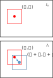
\includegraphics[width=\columnwidth]{./images/optical_flow/klt_tracking.pdf}
      \end{center}
    \end{column}
    \begin{column}{0.7\textwidth}  %%<--- here
      \[
      SSD(u,v) = \sum_{x,y \in \Omega} \big(I_0(x,y) - I_1(x+u, y+v)\big)^2
      \]

      \[
      \approx \sum ( I_0(x,y) - I_1(x,y) - I_x u - I_y v )^2
      \]

      \[
      \Rightarrow SSD(u,v) = \sum ( \Delta I - I_x u - I_y v )^2
      \]
    \end{column}
  \end{columns}
  References:  
  Lucas \& Kanade (1981), Tomasi \& Kanade (1991)
\end{frame}

% Slide 16
\begin{frame}{The Kanade-Lucas-Tomasi (KLT) tracker}
  To minimize it, we differentiate with respect to $(u,v)$ and equate to zero:
  
  \[
  \frac{\partial SSD}{\partial u} = 0, \quad \frac{\partial SSD}{\partial v} = 0
  \]
  
  This yields a system of linear equations.
\end{frame}

% Slide 17
\begin{frame}{The Kanade-Lucas-Tomasi (KLT) tracker}
  Linear system of two equations in two unknowns, written in matrix form:
  
  \[
  \begin{bmatrix}
    I_x^2 & I_x I_y \\
    I_x I_y & I_y^2
  \end{bmatrix}
  \begin{bmatrix}
    u \\ v
  \end{bmatrix}
  =
  \begin{bmatrix}
    I_x \Delta I \\ I_y \Delta I
  \end{bmatrix}
  \]
  
  Haven’t we seen this matrix already? Recall Harris detector!
\end{frame}

% Slide 18
\begin{frame}{The Kanade-Lucas-Tomasi (KLT) tracker}
  In practice, $\det(M)$ should be non-zero, which means eigenvalues should be large.  
  That is, the region should be a corner or textured region (not flat, not an edge).
  
  % \begin{figure}
  %   \centering
  %   \fbox{\includegraphics[width=0.7\textwidth]{placeholder.png}}
  % \end{figure}
\end{frame}

% Slide 10
\begin{frame}
  \frametitle{Lucas-Kanade Method}
  \textbf{Assumption:} Optical flow is constant in a small neighborhood.

  Formulate system of equations and solve using least squares.

  \vspace{0.5cm}
  \centering
  % \includegraphics[width=0.6\textwidth]{placeholder-slide25.png}
\end{frame}

% Slide 11
\begin{frame}
  \frametitle{When Does Optical Flow Estimation Work?}
\begin{itemize}
  \item Smooth regions: Bad (small eigenvalues).
  \item Edges: Bad (aperture problem).
  \item Textured regions: Good (large, diverse gradients).
\end{itemize}

\vspace{0.5cm}
\centering
% \includegraphics[width=0.6\textwidth]{placeholder-slide32.png}
\end{frame}

% Slide 12
\begin{frame}
  \frametitle{Large Motion: Problem}
Taylor approximation invalid when displacements are large.

\vspace{0.5cm}
\centering
% \includegraphics[width=0.6\textwidth]{placeholder-slide34.png}
\end{frame}

% Slide 13
\begin{frame}
  \frametitle{Coarse-to-Fine Estimation}
Use resolution pyramid:
\begin{itemize}
  \item Compute flow at low resolution.
  \item Warp and refine at higher resolutions.
  \item Repeat until full resolution.
\end{itemize}

\vspace{0.5cm}
\centering
% \includegraphics[width=0.6\textwidth]{placeholder-slide36.png}
\end{frame}

% Slide 14
\begin{frame}
  \frametitle{Alternative Approach: Template Matching}
\begin{itemize}
  \item Use template window from one frame.
  \item Search for best match in next frame.
  \item Difference gives optical flow.
  \item Slow and can produce mismatches.
\end{itemize}

\vspace{0.5cm}
\centering
% \includegraphics[width=0.6\textwidth]{placeholder-slide41.png}
\end{frame}

% Slide 15
\begin{frame}
  \frametitle{Applications of Optical Flow}
\begin{itemize}
  \item Optical mouse: motion tracking.
  \item Traffic monitoring: estimate vehicle speed.
  \item Video retiming: slow motion.
  \item Stabilization: remove camera shake.
  \item Face tracking: expressions, blinking.
\end{itemize}

\vspace{0.5cm}
\centering
% \includegraphics[width=0.6\textwidth]{placeholder-slide47.png}
\end{frame}

% References
% \begin{frame}
%   \frametitle{References}
%     \tiny
%     [Barron 2005] J. L. Barron, D. J. Fleet, and S. Beauchemin, IJCV 2005. \\
%     [Black 1993] M. J. Black and P. Anandan, ICCV 1993. \\
%     [Bouguet 2000] J. Y. Bouguet, Intel Tech Report 2000. \\
%     [Brox 2004] T. Brox, A. Bruhn, N. Papenberg, J. Weickert, ECCV 2004. \\
%     [Horn 1981] B. K. P. Horn and B. G. Schunck, AI 1981. \\
%     [Liu 2014] S. Liu, L. Yuan, P. Tan, J. Sun, CVPR 2014. \\
%     [Lucas 1981] B. D. Lucas and T. Kanade, Imaging Workshop 1981.
% \end{frame}